%% Submissions for peer-review must enable line-numbering 
%% using the lineno option in the \documentclass command.
%%
%% Preprints and camera-ready submissions do not need 
%% line numbers, and should have this option removed.
%%
%% Please note that the line numbering option requires
%% version 1.1 or newer of the wlpeerj.cls file, and
%% the corresponding author info requires v1.2

\documentclass[fleqn,10pt,lineno]{wlpeerj} % for journal submissions
% \documentclass[fleqn,10pt]{wlpeerj} % for preprint submissions
\usepackage{gensymb} %\degree


\title{Show the model! -- Combining data, distribution summary, model effects, and uncertainty in a single plot}

\author[1]{Jeffrey A. Walker}
%\author[2]{Second Author}
\affil[1]{Department of Biological Sciences, University of Southern Maine, 70 Falmouth St., Portland, ME 04103}
%\affil[2]{Address of second author}
\corrauthor[1]{Jeffrey A. Walker}{walker@maine.edu}

% \keywords{Keyword1, Keyword2, Keyword3}

\begin{abstract}
Dummy abstract text. Dummy abstract text. Dummy abstract text. Dummy abstract text. Dummy abstract text. Dummy abstract text. Dummy abstract text. Dummy abstract text. Dummy abstract text. Dummy abstract text. Dummy abstract text.
\end{abstract}

\begin{document}

\flushbottom
\maketitle
\thispagestyle{empty}

\section*{Introduction}
Recommended best practices for the reporting of statistical results include 1) showing the raw data and/or distribution of data in plots \citep{Drummond_Show_2011,Weissgerber_Bar_2015,Spitzer_BoxPlotR_2014,Krzywinski_Points_2014,Harrell_Statistical_2002,Weissgerber_Transparent_2016} and focusing on 2) effect size and (3) uncertainty in effect estimates instead of $p$-values of null hypothesis tests \citep{Nakagawa_Effect_2007, Yoccoz_Use_1991, Johnson_insignificance_1999, Curran-Everett_Fundamental_1998}. By contrast, standard practice throughout experimental biology includes the reporting of ANOVA results in tables and treatment means and standard errors of the mean in plots. At best, ANOVA tables poorly communicate effect size and uncertainty. Effects and uncertainty can be inferred from plots of treatment means and standard errors only indirectly.

Here, I introduce the Harrell plot, a tool to communicate statistical results from experiments, or any analysis with categorical independent variables (ANOVA-like linear models). A Harrell plot combines 1) a dot plot to show individual values, 2) a box plot to show the distribution of the response within treatment groups, and 3) a forest plot of effect estimates and confidence intervals to show modeled effect sizes and uncertainty. The combination of the effects in the top part and distribution in the bottom part of a Harrell plot was inspired by Fig. 1.1 of \cite{Harrell_Statistical_2002}. The Harrell plot is implemented both as an online HarrellPlot Shiny app for users with no or limited R experience, including undergraduate biology majors, and the R package HarrellPlot, for users with some R experience. 

\subsection*{Effect size and uncertainty}
By effect, or effect size, I mean the magnitude and direction of the difference in response to some treatment, or some combination of treatments. If the mean critical thermal minimum is 5.1 \degree C in the control group of flies and 5.8 \degree C in the treated group, then the effect is $5.8 \degree \textrm{C} - 5.1 \textrm{C} = +0.7 \degree \textrm{C}$. The non-intercept coefficients of a linear model are effects. Contrasts of a linear model are effects. A confidence interval of the effect is a measure of the uncertainty in the estimate.  A 95\% confidence interval of the effect has a 95\% probability (in the sense of long-run frequency) of containing the true effect. This probability is a property of the population of intervals that could be computed using the same sampling and measuring procedure. It is not correct, without further assumptions, to state that there is a 95\% probability that the true effect lies within the interval. However, if we have only weak prior beliefs about the possible values of the effect, then it is valid, though possibly misleading, to state that there is an approximately 95\% probability that the true effect lies in the interval \citep{Greenland_Living_2013, Gelman_Values_2013}. Perhaps a more useful interpretation is that the interval contains the range of effects that are consistent with the data, in the sense that a $t$-test would not reject the null hypothesis of a difference between the estimate and any value within the interval (this interpretation does not imply anything about the true value).

While many experiments in biology are conducted with a proximate goal of discovering or confirming that an effect exists (that is, the effect is something other than zero), the ultimate goal of a research program should be to understand the biological (including clinical, behavioral, ecological or evolutionary) consequences of effects \citep{Yoccoz_Use_1991, Curran-Everett_Fundamental_1998, Nakagawa_Effect_2007, Batterham_Making_2006}. These consequences are functions of effect magnitude and direction and, consequently, estimates of effect size and uncertainty are tools for these ultimate goals. By contrast, hypothesis testing and $p$-values are tools only for the more proximate goal of effect presence. Importantly, the discovery that an effect exists requires more than a $p$-value, including both replicate experiments and modified experiments that ``probe their experimental systems in multiple, independent ways''  (\citealp{Vaux_Research_2012}, see also \citealt{Munafo_Robust_2018}). Probing is standard in much of cell and molecular biology \citep[but see][]{KaelinJr_Publish_2017}. Replications are uncommon throughout most of experimental biology. It probably cannot be emphasized enough that finding statistically significant $p$-values is a very low-bar in experimental biology. All components of complex physiological systems are causally connected and perturbing any feature of a system will have some effect on everything, however small (this may not be true in a simplified experimental system with a minimal number of components). Consequently, Type I errors will not exist in complex systems and the concept of null-hypothesis testing becomes meaningless. Instead, researchers should be concerned with sign and magnitude errors (xxx) and with conditional dependencies.

Confidence intervals of effects can be (and are most often) used to infer ``statistical significance''. Statisticians have long advocated for the far more valuable use of a confidence interval as a tool to infer the sensitivity of an interpretation or conclusion to the data \citep{Tukey_Philosophy_1991}. Again, a confidence interval of an effect gives the range of parameter values that are consistent with the data \citep{Amrhein_earth_2017b}. Consequently, as evidence for a theory in academic biology or a decision in applied biology, the whole range of values within a confidence interval, and not just the mean or median, should be consistent with an interpretation or conclusion, otherwise the data are ambiguous (or "inconclusive", but this might suggest that the results from a single study could ever be "conclusive"). One scheme for implementing this strategy is shown in Figure~\ref{fig:interpretation}, which is a modification of Figure 2 of \cite{Barker_Inference_2008}, which itself is a corrected interpretation of Figure 2 in \cite{Batterham_Making_2006}.

\subsection*{Mean-and-error plots}
Figure~\ref{fig:one}A and B illustrate two kinds of mean-and-error plot. The unpublished data are the maximum burst speed of \textit{Drosophila melanogaster} individuals from two lines that have undergone selection in a compartmentalized wind tunnel (weber, marden xxx) and two control lines. Maximum burst speed was measured on individual flies that were stimulated to take-off and fly against a wind of known speed in a wind tunnel (detailed methods are given in Supplement xxx). The mean response of a group is represented either by the height of the bar (A) or a point symbol (B). The error bar most commonly represents one standard error of the mean; a confidence interval is less common. Occasionally, the error bar represents one sample standard deviation. Bar-and-error plots are ubiquitous in experimental cell biology. Point-and-error plots are more common in animal physiology than in cell biology. Perhaps because of the ubiquity of bar plots in cell biology (including the pages of Science, Nature, and Cell), most criticism of mean-and-error plots focusses on bar plots, which are pejoratively called ``dynamite'', ``plunger'', or ``antenna'' plots.

\begin{figure}[]
\begin{center}
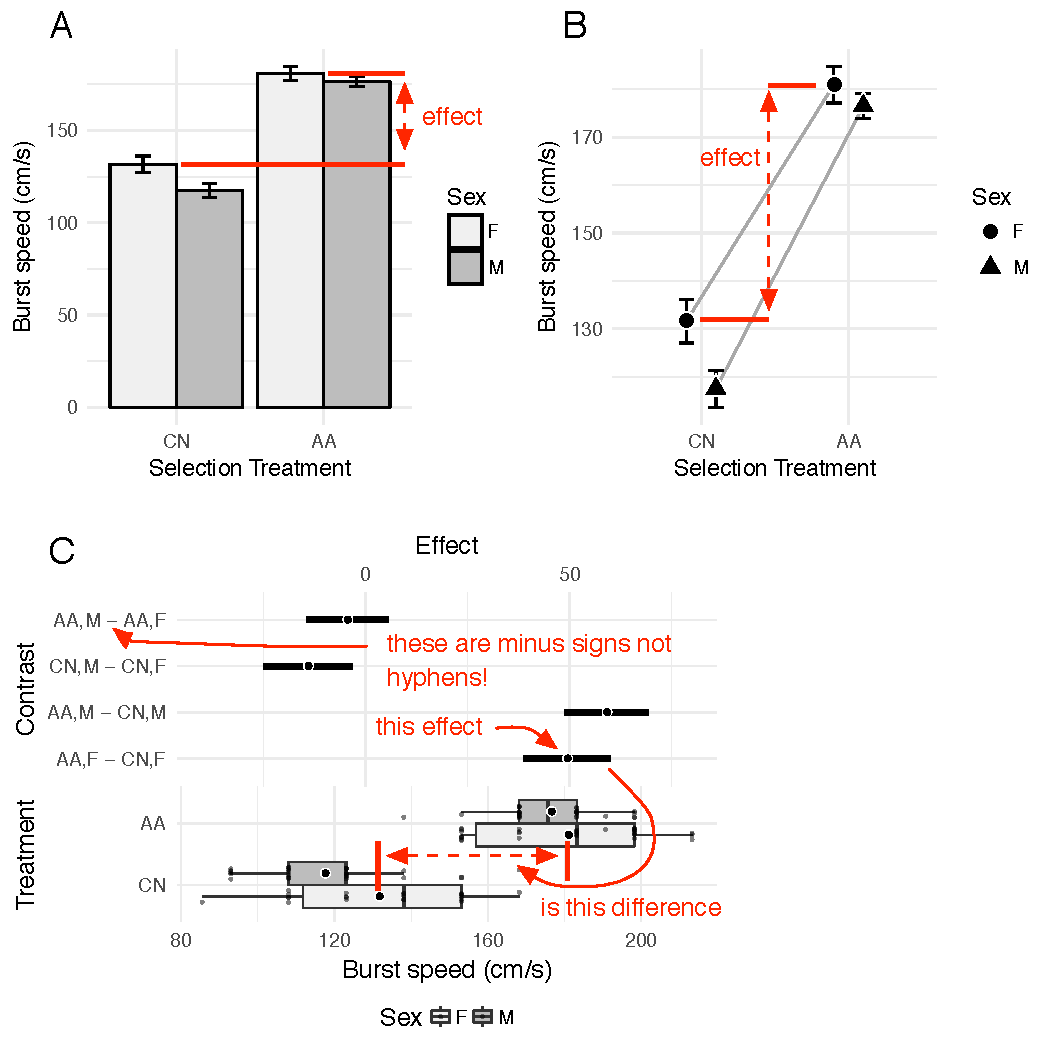
\includegraphics[width=4 in]{figs/fig1}
\caption{Three methods for communicating results of an experiment. In the bar plot (A) and the dot plot (B), the treatment effect is inferred by mentally computing the distance between treatment means. In the Harrell plot (C), the treatment effect is plotted in addition to the treatment means. Key: AA selected flies, CN control flies, F female, M male}
\label{fig:harrell}
\end{center}
\end{figure}

Three, related criticisms of mean-and-error plots are \citep{Drummond_Show_2011,Weissgerber_Bar_2015,Rousselet_few_2016}, first, they do not show the data, which is important because multiple distributions can produce the same mean and error. Second, mean-and-error plots typically fail to reflect the analyzed model. For example, almost all mean-and-SE plots illustrate standard errors computed independently in each group instead of pooled standard errors resulting from the model. Or, for clustered data (repeated measures, blocked designs) mean-and-error plots give no indication of this lack of independence. And, third, error bars based on the sample standard deviation or standard error of the mean are not easily interpretable, and suggest a false interpretation, if the underlying data are not approximately normal.

These criticisms and even the solutions (box plots or dot plots) do not address the elephant in the room -- mean-and-error plots only indirectly communicate what we often want to directly communicate: the effects of the experimental treatments and the uncertainty in these effects. In a mean-and-error plot, effects can be mentally reconstructed by comparing the difference in the response between two groups (Figure~\ref{fig:one}A and B). This is relatively easy if there are few groups and if the differences are large relative to the scale of the response axis. In bar plots especially, differences can often be very small relative to the height of the bar and Figure~\ref{fig:one}A is a good example of this. Regardless, effect uncertainty is much harder to mentally reconstruct, because the proper interval is a function of a standard error that is itself a function of the distribution of error variance in multiple groups. Because the approximate end-points of a confidence interval of a difference is time-consuming to mentally construct, mean-and-error plots encourage focus on the presence/absence of an effect (and it's direction) instead of the magnitude of the effect, including the magnitude of the ends of the confidence interval.

\subsection*{The Harrell plot}
The Harrell plot addresses all three recommended practices by combining a forest plot of treatment effects, a box plot, and a jittered dot plot, into a single plot (Figure~\ref{fig:one}C). Modeled effects are illustrated in the upper part of the plot using a dot symbol representing the effect estimate and horizontal bars representing the effect uncertainty (Figure~\ref{fig:one}C). Here, the bars are 95\% confidence intervals but these could be credible intervals from a Bayesian analysis. Forest plots of effects with horizontal uncertainty intervals are common in analyses with multiple responses, in meta-analysis, and in the epidemiology literature. The illustrated effects can be the coefficients of the linear model or contrasts between treatment combinations. If contrasts, these can be comparisons with a reference (such as a control) or pairwise comparisons.

The raw data are shown in the lower part of the plot using jittered dots, clustered by group. The distribution of data in each group is also shown in the lower part of the plot using a box plot. The precise tool to show the data and distributions is flexible but jittered dots and box plot reflect the best practice for much of experimental biology. While some advocate the use of an error bar, the box plot is more informative than an interval based on the sample standard deviation (including the sample confidence interval). And, an interval based on the standard error of the mean (including a 95\% confidence interval of the mean) is often not the uncertainty that we want to communicate (see \textit{Effect size and uncertainty} above).

\subsection*{Using a Harrel plot}

The major advantage of a Harrell plot over bar plots and Cleveland dot plots is the direct communication of modeled effects.


1) modeled effects

2) nudges

which shows the effects of mean developmental temperature ($dev.temp$) and daily fluctuation in temperature ($dev.treat$) on the critical thermal minimum ($CT_{min}$) in \textit{Drosophila melanogaster} (xxx). In both the results and discussion, the authors emphasized the 0.3 -- 0.4 effect size, a statistic which is directly communicated by Harrell but not the mean-and-error plot. The authors also emphasized the point that the fluctuation treatment effect is much smaller than the developmental temperature effect. While a comparison of the point estimate of the effect is fairly easy to mentally compute from the mean-and-error plot, it is much harder to infer the sensitivity of this conclusion to the data using a mean-and-error plot because for this inference we need the effect uncertainty. Using the Harrell plot, it is easy to see that the the upper ends of the intervals for the fluctuation treatment (the top two intervals in Figure~\ref{fig:one}C) are well below the lower ends of the intervals for the temperature treatment (the bottom two intervals in Figure~\ref{fig:one}C) and, consequently, the conclusion of a much smaller fluctuation-treatment effect is not sensitive to sampling error.

The Harrell plot also shows effects that are broadly similar. For example, Figure~\ref{fig:bee} shows the effects of a juvenile starvation treatment ($Juv.starve$) and adult starvation duration ($Ad.starve$) on metabolic rate in honey bee (\textit{Apis melifera}) (the data are not publicly available and were simulated to closely mimic the published figure) (xxx). A visual comparison of the effect of juvenile starvation in the long-adult-starvation bees (top-most effect in the plot) and of the effect of the adult starvation treatment in the control bees (bottom-most effect in the plot) shows that both effects and their confidence intervals are nearly identical. Consequently, the statistical evidence for making inference about these effects is effectively the same for both. I specifically used this example because the $p$-values for the two effects are 0.063 and 0.046 respectively (the reported $p$-values were 0.06 and 0.045). Unfortunately, it is standard procedure in experimental biology to use these $p$-values to intrepret this as ``no effect'' and ``effect'' -- an absurd practice that has long been criticized by statisticians and is a gross distortion of the original usage of Type I error rates in hypothesis testing (xxx). 

Confidence intervals that border zero present interpretation ambiguities because this pattern implies that (possibly trivially) small values of the true difference are consistent with the data.

1. coefficients vs. contrast
2. raw vs. percent vs. standardized
3. comparison of effects  - p value vs. effect(fly thermal data)
2) negative values not apparent in bar plot without data (xxx data)
3) mean CI raw vs. model (moss data?)

- "no effects" not consistent with intervals. (p > 0.05)
- big effect if interval barely outside of zero. data? (related but p < 0.05)
- urchin data - interaction interval consistent with both hypotheses.
- moss data - SEMs don't reflect analysis.


\subsection*{show the data}
outliers - thermal limits
below zero - xxx

\subsection*{box plot}
distribution suggesting glm




\section*{Acknowledgments}

So long and thanks for all the fish.

\bibliography{hplot}

\end{document}